\subsection{Bilanzräume in Organisationen des tertiären Wirtschaftssektors}

%%%%%%%%%%%%%%%%%%%%%%%%%%%%%%%%%%%%%%%%%%%%%%%%%%%%%%%%%%%%%%%%%%%%%%%%%%%%%%%%%%%%%%%%%%%%%%%%%%%%%%%%%%%%%%%%%%%%%%%%%%%%%%%%%%%%%%%%%%%%%%%%%%%%%%%%%%%%%%%%%%%

\subsubsection{System- und Bilanzraumgrenzen}
Eine Bilanz bezieht sich gemäß Ahrendts (2014, Kapitel 1.5) auf das von der Systemgrenze eingeschlossene Kontrollgebiet. Die Systemgrenze kann dabei unter Berücksichtigung 
der Zweckmäßigkeit frei definiert werden (\cite[Kapitel 1.5]{Ahrendts.2014}).
Das definierte System kann auch als Bilanzraum bezeichnet werden, da die Berechnung der in einen Bilanzraum ein- und austretenden Ströme als Bilanzierung bezeichnet wird 
(\cite[S. 65]{Rönsch.2015}).
Einen Ansatz zur Definition von Bilanzräumen liefert Miller (2016, S. 105) mit der Konkretisierung von Bewertungsräumen mittels Kriterien der Bilanzgrenze, dem 
Aggregationsniveau und der Bewertungseinheit. Das definierte System dient der Bewertung der Nutzung der Ressourcen, wobei der Effizienzbegriff eine zentrale Rolle spielt 
(\cite[S. 107]{Miller.2016}).
Miller (2016, S. 107) definiert die Effizienz nach Gleichung \eqref{EffizienzgleichungMiller}.

\begin{equation}
    \text{Effizienz} := \frac{\text{Erreichter Nutzen}}{\text{Aufwand}}
    \label{EffizienzgleichungMiller}
\end{equation}

Der Aufwand umfasst nach Miller (2016, S. 108f.) unterschiedliche Ressourcen, wobei im Kontext energiewirtschaftlicher Fragestellungen der Fokus auf der Ressource Energie liegt.
Der Nutzen ist vom Untersuchungsgegenstand abhängig und wird im Kontext der energiewirtschaftlichen Fragestellung häufig über Energiedienstleistungen operationalisiert (\cite[S. 107]{Miller.2016}). Betrachtet man, dass der Nutzen grundsätzlich durch Befriedigung von Bedürfnissen beschrieben wird, entsteht im Kontext der Energiewirtschaft ein Nutzenergiebedarf zur Befriedigung der Bedürfnisse im Rahmen einer Energiedienstleistung (\cite[S. 107]{Miller.2016}).
Sowohl die Ressourcen des Aufwands als auch die Energiedienstleistung auf der Nutzenseite werden durch eine Bewertungseinheit formalisiert (\cite{Miller.2016}).
Der Nutzen wird meist implizit durch den gewählten Untersuchungsgegenstand definiert (\cite[S. 110]{Miller.2016}).
Die in \eqref{EffizienzgleichungMiller} aufgestellte Nutzen-Aufwand-Relation stellt die Grundlage der Definition der Bilanzraumgrenze dar.
Die Bilanzraumgrenze lässt sich somit in die aufwandsseitige Bilanzgrenze, die alle zu bilanzierenden Ressourcen umfasst, und die nutzenseitige Bilanzgrenze, die sich auf die zu bilanzierende Energiedienstleistung bezieht (\cite[S. 111]{Miller.2016}).

Das von Miller (2016) beschriebene Konzept bringt eine neue Perspektive auf die in \eqref{BilanzierungsgleichungAhrendt} und \eqref{BilanzierungsgleichungAhrendtStrom} 
aufgestellte Bilanzgleichung. Sie bringt das Prinzip der Effizienz ein und teilt eine Bilanz in Aufwands- und Nutzenseite.
Aufwandsseitig sind die in \eqref{BilanzierungsgleichungAhrendt} zufließenden Ströme, also die dem System zugeführten Ressourcen der Zustandsgröße, zu betrachten.
Nutzenseitig müssen abfließende Ströme, also die aus dem System fließende Energie zur Befriedigung der Energiedienstleistung der Zustandsgröße, betrachtet werden.
Die abfließenden Ströme werden nach Energiedienstleistung mit Nutzengrößen operationalisiert (\cite{Miller.2016}).

%%%%%%%%%%%%%%%%%%%%%%%%%%%%%%%%%%%%%%%%%%%%%%%%%%%%%%%%%%%%%%%%%%%%%%%%%%%%%%%%%%%%%%%%%%%%%%%%%%%%%%%%%%%%%%%%%%%%%%%%%%%%%%%%%%%%%%%%%%%%%%%%%%%%%%%%%%%%%%%%%%%

\subsubsection{Untersuchungsgegenstand und Nutzengrößen}

In dieser Forschung bezieht sich der Untersuchungsgegenstand aufgrund der Verortung der Organisationen im tertiären Wirtschaftssektor auf Gebäudeenergie. 
Es müssen also auf der Grundlage dieses Untersuchungsgegenstands angemessene Nutzengrößen mit entsprechenden Bewertungseinheiten erfasst werden.
Da auch die Definition der Systemgrenze vom Untersuchungsgegenstand beeinflusst wird (\cite[S. 109]{Miller.2016}), gilt die Zweckmäßigkeit der Systemgrenze auch für die 
zu untersuchenden Nutzengrößen.
Die DIN EN ISO 50001:2018-12 gibt mit dem Ziel der fortlaufenden Verbesserung der energiebezogenen Leistung eine Vorgabe zur zweckmäßigen Definition der Nutzengröße 
(\cite[S. 11]{DIN50001.2018}).
Die Vornorm DIN V 18599-1:2018-09, herausgegeben vom Deutschen Institut für Normung e. V. (2018, S. 1), behandelt die energetische Bewertung von Gebäuden und stellt ein 
Verfahren zur Durchführung der Gesamtenergiebilanz bereit (\cite[S. 9]{DIN18599.2018}). Ihre Ausrichtung auf die energetische Bewertung erfüllt die Zweckmäßigkeit der 
DIN EN ISO 50001:2018-12. Der Fokus auf die Bewertung von Gebäuden entspricht der Zielsetzung der DIN V 18599-1:2018-09.

Im Rahmen der energetischen Bewertung von Gebäuden betrachtet die DIN V 18599-1:2018-09 die Bilanzierung des Nutz-, End- und Primärenergiebedarfs (\cite{DIN18599.2018}).
In einem energiewirtschaftlichen Rahmen hat besonders der Nutzenergiebedarf eine große Bedeutung, da er aus der Befriedigung der Bedürfnisse im Rahmen einer 
Energiedienstleistung resultiert (\cite[S. 107]{Miller.2016}).

\begin{figure}[H]
    \centering
    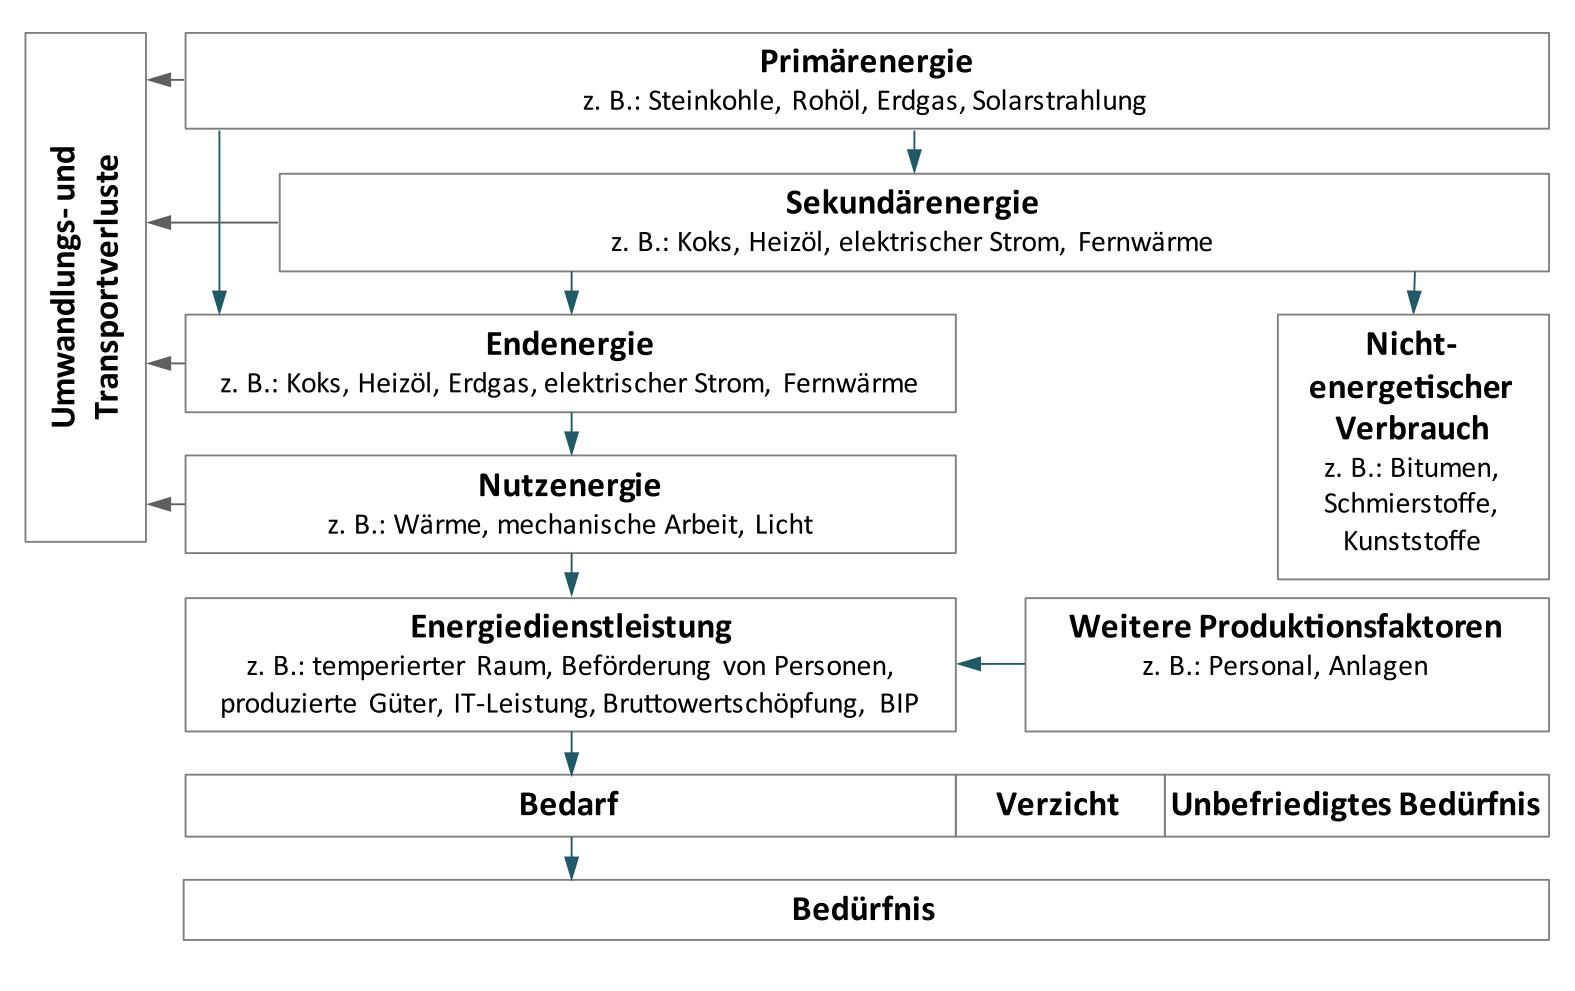
\includegraphics[width=1\textwidth]{../../Ressourcen/Abbildungen/Energiefluss_Miller.jpg}
    \caption{Energieflussschema. (Dargestellt von Miller (2016))}
    \label{fig:Energieflussschema_Miller}
\end{figure}

Betrachtet man die Abbildung \eqref{fig:Energieflussschema_Miller}, so stellt man fest, dass die Nutzenergie aus Endenergie umgewandelt wird.
Außerdem wird nach Abbildung \eqref{fig:Energieflussschema_Miller} die Nutzenergie in Energiedienstleistungen umgewandelt.
Da die Endenergie die Energiemenge ist, die dem Bilanzraum zur bestimmungsgemäßen Nutzung bereitgestellt wird (\cite[Kapitel 3.1.2]{DIN18599.2018}), 
repräsentiert diese Energieform die Menge der potenziellen Ressourcen auf der Aufwandsseite der Bilanzierung.
Außerdem wird der praktische Sachverhalt veranschaulicht, dass bei der Umwandlung von Endenergie in Energiedienstleistungen über die Nutzenergie 
Umwandlungs- und Transportverluste berücksichtigt werden müssen.

Die DIN V 18599-1:2018-09 definiert die Heizung, Kühlung, Lüftung, Trinkwarmwasseraufbereitung und Beleuchtung von Gebäuden oder Gebäudezonen 
als relevante Nutzengrößen zur energetischen Bewertung von Gebäuden (\cite{DIN18599.2018}).
Somit wird im von Miller (2016) aufgestellten Konzept der Nutzenergiebedarf der jeweiligen Nutzengröße durch die Nutzenergie gedeckt und muss 
je nach Nutzengröße unterschiedlich definiert werden. Die Nutzenergie wird im Konzept von Miller (2016) durch die Ressourcen repräsentiert.
Im Rahmen der Vornorm wird der Nutzenergiebedarf als Überbegriff für Nutzwärmebedarf, Nutzkältebedarf, Nutzenergiebedarf für Trinkwarmwasser, 
Beleuchtung und Befeuchtung definiert (\cite[Kapitel 3.1.3]{DIN18599.2018}).
Der jeweilige Nutzenergiebedarf muss durch Nutzenergie gedeckt werden, welche von der DIN V 18599-1:2018-09 je nach Art des Nutzenergiebedarfs 
wie folgt definiert wird.

\begin{itemize}
    \item \textbf{Nutzenergie für Beleuchtung}: Die Energiemenge, die zur Ausreichenden Beleuchtung des Gebäudes beziehungsweise der Gebäudezone 
    aufgewendet werden muss (\cite[Kapitel 5.3.1]{DIN18599.2018}).
    \item \textbf{Wärmeenergie}: Die Wärmemenge, die dem Gebäude beziehungsweise der Gebäudezone zusätzlich (bedarfs-)geregelt zugeführt wird, 
    um die vorgegebene Sollinnentemperatur einzuhalten (\cite[Kapitel 5.3.1]{DIN18599.2018}).
    \item \textbf{Kälteenergie}: Die Kälteeinträge, die dem Gebäude bzw. der Gebäudezone zusätzlich (bedarfs-)geregelt zugeführt werden, um die 
    vorgegebene Sollinnentemperatur einzuhalten (\cite[Kapitel 5.3.1]{DIN18599.2018}).
    \item \textbf{Nutzenergie für die Trinkwarmwasserbereitung}: Die Energiemenge, die zum Erwärmen, Kühlen, Befeuchten und Entfeuchten der 
    Luft in einer raumlufttechnischen Anlage zu- bzw. abgeführt werden muss, um den erforderlichen Zuluftzustand zu erreichen (\cite[Kapitel 5.3.1]{DIN18599.2018}).
    \item \textbf{Nutzenergie für die Luftaufbereitung}: Die Energiemenge, die zum Erwärmen, Kühlen, Befeuchten und Entfeuchten der Luft in 
    einer raumlufttechnischen Anlage zu- bzw. abgeführt werden muss, um den erforderlichen Zuluftzustand zu erreichen (\cite[Kapitel 5.3.1]{DIN18599.2018}).
\end{itemize}

Abbildung \eqref{fig:Übersicht_Bilanzräume} ordnet die mithilfe der DIN V 18599-1:2018-09 erfassten Nutzengrößen des Untersuchungsgegenstands in das von 
Miller (2016) erarbeitete Konzept der Bewertungsräume ein.

\begin{figure}[H]
    \centering
    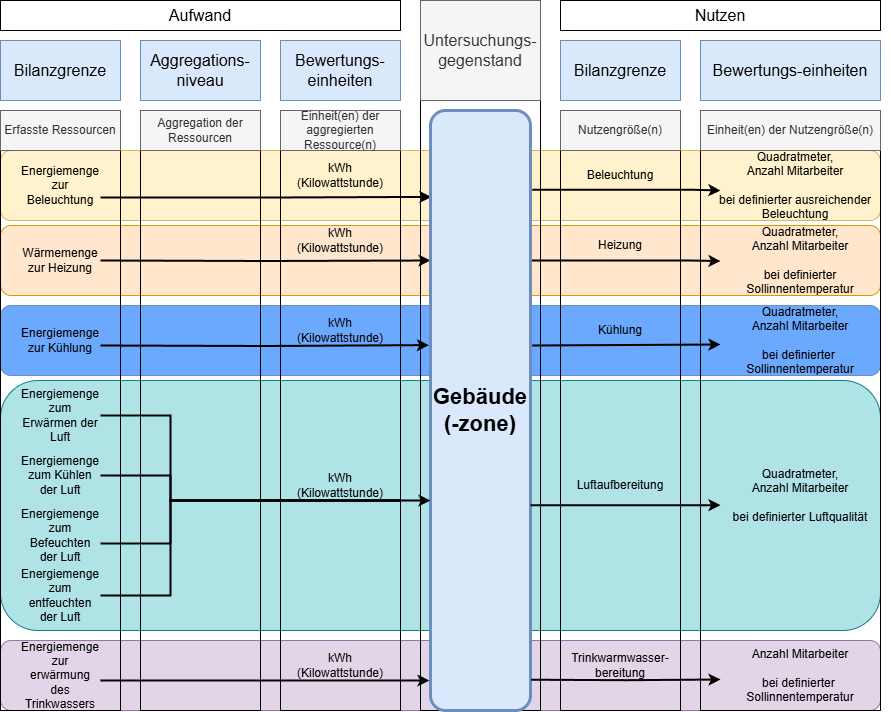
\includegraphics[width=1\textwidth]{../../Ressourcen/Abbildungen/Nutzengröße_Bewertungseinheit.png}
    \caption{Bilanzrgrenzen Aufwandsseitig/Nutzenseitig. (Eigene Darstellung basierend auf Miller (2016) und DIN V 18599-1:2018-09 (2018))}
    \label{fig:Übersicht_Bilanzräume}
\end{figure}

%%%%%%%%%%%%%%%%%%%%%%%%%%%%%%%%%%%%%%%%%%%%%%%%%%%%%%%%%%%%%%%%%%%%%%%%%%%%%%%%%%%%%%%%%%%%%%%%%%%%%%%%%%%%%%%%%%%%%%%%%%%%%%%%%%%%%%%%%%%%%%%%%%%%%%%%%%%%%%%%%%%

\subsubsection{Energieströme und Bewertungseinheiten}

In Gleichung \eqref{BilanzierungsgleichungAhrendt} wird zwischen in das System zu- und abfließenden Strömen der Zustandsgröße unterschieden.
Die zufließenden Ströme können als Ressourcen der Aufwandsseite im von Miller (2016) aufgestellten Konzept der Bewertungsräume 
betrachtet werden, wobei energetische Ressourcen im Vordergrund stehen. Aufwandsseitige Ressourcen können zu einer Ressource mit 
einer Bewertungseinheit zusammengefasst werden (\cite[S. 112]{Miller.2016}). Sollten nach Erfassung und optionaler Aggregation der 
Ressourcen mehrere Ressourcenkategorien bestehen, können diese mit unterschiedlichen Bewertungseinheiten bilanziert werden (\cite[S. 112]{Miller.2016}). 
Im Rahmen dieser Forschungsarbeit werden aufwandsseitig ausschließlich Energieressourcen betrachtet.
Die aufwandsseitigen Ressourcen haben die Bewertungseinheit: kWh und deren Vielfaches, da diese Einheit bei Energiebilanzen in der Regel 
für alle Energieformen bevorzugt verwendet wird (\cite[S. 65]{Konstantin.2023}). Die aufwandsseitige Bewertungseinheit kWh lässt sich problemlos in 
die Einheit der Zustandsgröße der betrachteten Bilanzräume: Joule überführen.

Die abfließenden Ströme in \eqref{BilanzierungsgleichungAhrendt} werden durch die Nutzenseite des von Miller (2016) aufgestellten Konzepts repräsentiert.
Um die Nutzenseite abzubilden, ist eine Konkretisierung der Energiedienstleistung durch eine angemessene Bewertungseinheit, welche vom Untersuchungsgegenstand 
impliziert wird, notwendig (\cite{Miller.2016}). Diese Bewertungseinheit ist keine Energieeinheit und kann beispielsweise bei der Untersuchung der Temperierung 
von Räumen die Quadratmeteranzahl des Bilanzraums bei einer definierten Soll-Temperierung sein (\cite{Miller.2016}). Die Nutzenseite lässt sich folglich schwer 
in die Bewertungseinheit der Zustandsgröße: Joule überführen.

%%%%%%%%%%%%%%%%%%%%%%%%%%%%%%%%%%%%%%%%%%%%%%%%%%%%%%%%%%%%%%%%%%%%%%%%%%%%%%%%%%%%%%%%%%%%%%%%%%%%%%%%%%%%%%%%%%%%%%%%%%%%%%%%%%%%%%%%%%%%%%%%%%%%%%%%%%%%%%%%%%%

\subsubsection{Energiequellen und -senken}
Gleichung \eqref{BilanzierungsgleichungAhrendt} unterscheidet zwischen Quellen, Senken und zu- beziehungsweise abfließenden Strömen der Zustandsgröße.
Quell- und Senkenströme treten in einer Energiebilanz nach dem ersten Hauptsatz der Thermodynamik nicht auf, da Energie eine Erhaltungsgröße ist (\cite[S. 14]{Ahrendts.2014}).
Im Rahmen der DIN EN ISO 50001:2018-12 bezieht sich der Begriff "Energie" auf verschiedene Arten von Energie, die erworben, gespeichert, aufbereitet, in einer Einrichtung oder einem Prozess verwendet
oder zurückgewonnen werden können (\cite[Kapitel 3.5.1]{DIN50001.2018}). Energie kann im Rahmen der Norm als Elektrizität, Brennstoff, Dampf, Wärme, Druckluft oder vergleichbares Medium auftreten
(\cite[Kapitel 3.5.1]{DIN50001.2018}).
Folglich werden alle Energieströme, in denen Energie in eine Energieform umgewandelt wird, die nicht die genannten Kriterien erfüllt, als Energiesenken betrachtet.
Analog dazu werden alle Energieströme, bei denen Energie, die nicht den von der Norm aufgestellten Kriterien entspricht, in eine nach ISO 50001 definierte Energieform
umgewandelt wird, als Energiequellen betrachtet.
In der Praxis stellen die in Abbildung \eqref{fig:Energieflussschema_Miller} dargestellten Umwandlungs- und Transportverluste Energiesenken dar. Energiequellen können beispielsweise
PV-Anlagen sein, da diese die Energie des Sonnenlichts, welche nach Definition der DIN EN ISO 50001:2018-12 nicht nutzbar ist, in nutzbare Energie umwandeln und als
Endenergie zur Verfügung stellen.

\subsubsection{Bilanzraumstrukturen}
Bisher wurde die strukturelle Definition von Bilanzräumen unter Berücksichtigung praktischer Herausforderungen gemäß der DIN EN ISO 50001:2018-12 in Organisationen 
des tertiären Wirtschaftssektors betrachtet. Eine Betrachtung der Beziehungen zwischen Bilanzräumen weist auch eine Relevanz zur Erfüllung der DIN EN ISO 50001:2018-12 auf.
So kann ein Bilanzraum in mehrere Teilbilanzräume zerlegt werden (\cite[S. 310]{Engelmann.2015}). Dies kann durch die Disaggregation in einzelne Prozesse, 
Anlagen oder räumlich getrennte Bereiche realisiert werden (\cite[S. 310]{Engelmann.2015}), wobei die Disaggregation in Prozesse bei Organisationen des tertiären 
Wirtschaftssektors eine geringere Relevanz hat.
Analog zur Zerlegbarkeit eines Bilanzraums lässt sich auch der Untersuchungsgegenstand eines Bilanzraums hierarchisch aufgliedern (\cite[S. 109]{Miller.2016}).
Die in Abbildung \eqref{fig:Übersicht_Bilanzräume} dargestellten Bilanzgrenzen für den Untersuchungsgegenstand Gebäude können also folglich in räumlich getrennte 
Gebäudezonen, wie zum Beispiel Etagen oder Räume, zerlegt werden. Dies ist beispielhaft in \eqref{fig:Disagggregation_Bilanzraum_Untersuchungsgegenstand} dargestellt.

\begin{figure}[H]
    \centering
    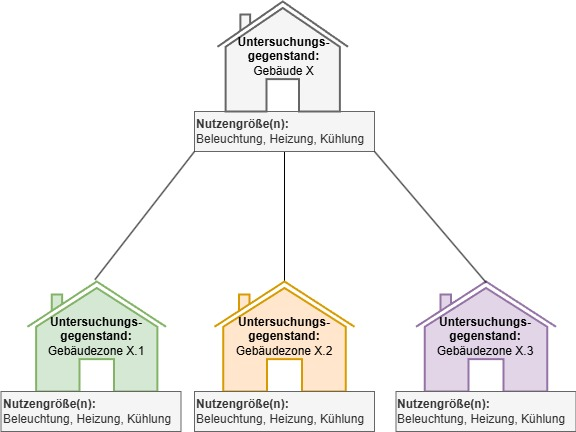
\includegraphics[width=0.8\textwidth]{../../Ressourcen/Abbildungen/Untersuchungsgegenstand_Zerlegt.jpg}
    \caption{Disagggregation eines Untersuchungsgegenstands. (Eigene Darstellung)}
    \label{fig:Disagggregation_Bilanzraum_Untersuchungsgegenstand}
\end{figure}

Zur Erfassung der Energiedaten einer Organisation bedarf es einer detaillierten und aussagekräftigen Analyse der Unterscheidung nach Verbrauchsarten 
(\cite[S. 14]{Hohnhold.2013}). Dabei ist die Disaggregation der Daten von der Größe der Organisation und dem Zweck der Analyse abhängig (\cite[S. 14f.]{Hohnhold.2013}).
Zur Analyse der Verbrauchsarten wäre es also auch denkbar, Bilanzräume anhand ihrer definierten Nutzengrößen zu disaggregieren.
In \eqref{fig:Disagggregation_Bilanzraum_Nutzengrößen} ist ein Beispiel für eine Disaggregation nach Nutzengrößen 
zur Analyse der Unterscheidung nach Verbrauchsarten visualisiert.




\begin{figure}[H]
    \centering
    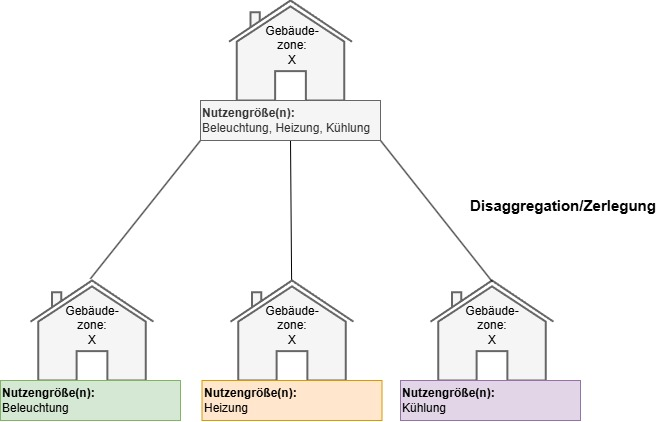
\includegraphics[width=0.8\textwidth]{../../Ressourcen/Abbildungen/Nutzengröße_Bewertungseinheit_Zerlegt.jpg}
    \caption{Disagggregation eines Bilanzraums nach Nutzengrößen. (Eigene Darstellung)}
    \label{fig:Disagggregation_Bilanzraum_Nutzengrößen}
\end{figure}